\documentclass{standalone}

\usepackage{tikz}
 \usetikzlibrary{shapes,shapes.misc,arrows}
 \tikzset{cross/.style={cross out, draw=black, minimum size=2*(#1-\pgflinewidth), inner sep=0pt, outer sep=0pt},
% %default radius will be 1pt. 
 cross/.default={2pt}}
\usepackage{amsmath}
\usepackage{fourier}

\begin{document}

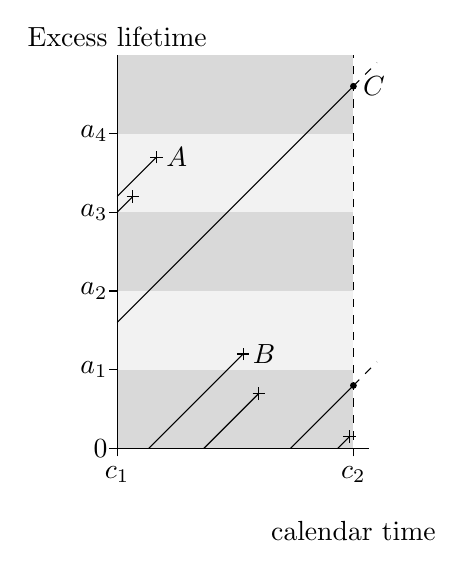
\begin{tikzpicture}
\fill [gray!10] (0,0) rectangle (3,5);
\fill [gray!30] (0,0) rectangle (3,1);
\fill [gray!30] (0,2) rectangle (3,3);
\fill [gray!30] (0,4) rectangle (3,5);
\draw[dashed](3,-0.1)--(3,5); %vertical right bar
% \draw[dotted, very thick, color=white](0,3.7)--(3,3.7);
% \draw[dotted, very thick, color=white](0,1.2)--(3,1.2);
% \draw(3.8,1.2)--(3.9,1.2) node[right] at (3.9,1.2) {\small $t_B$};
% \draw(3.8,0.8)--(3.9,0.8) node[right] at (3.9,0.8) {\small $c_2-x_D$};
% \draw(3.8,1.6)--(3.9,1.6) node[right] at (3.9,1.6) {\small $c_1-x_C$};
% \draw(3.8,3.2)--(3.9,3.2) node[right] at (3.9,3.2) {\small $c_1-x_A$};
% \draw(3.8,4.6)--(3.9,4.6) node[right] at (3.9,4.6) {\small $c_2-x_C$};
% \draw(3.8,3.7)--(3.9,3.7) node[right] at (3.9,3.7) {\small $t_A$};
% \draw (3.7,0)--(3.9,0) node[right]{\small $0$};

\node[anchor=base,inner sep=0pt, outer sep=0pt] at (0,5.1) {Excess lifetime};
\draw (0,0)--(3.2,0);
\draw (0,-0.1)--(0,5);
\node[below] at(0,-0.1) {$c_1$};
\node[below] at(3,-0.1) {$c_2$};
\node[left] at (0, 0) {$0$};
\draw (-0.1,0)--(0,0);
\draw (-0.1,1)--(0,1);
\draw (-0.1,2)--(0,2);
\draw (-0.1,3)--(0,3);
\draw (-0.1,4)--(0,4);
\node[left] at (0, 1) {$a_1$};
\node[left] at (0, 2) {$a_2$};
\node[left] at (0, 3) {$a_3$};
\node[left] at (0, 4) {$a_4$};
% \draw (2.2,0)--(2.2,-0.1) ;
% \draw (0.4,0)--(0.4,-0.1);
% \draw (-3.2,0)--(-3.2,-0.1);
% Draw C
\draw (0,1.6)-- (3,4.6);
\draw[dashed] (3,4.6) -- (3.3,4.9);
\draw[fill=black] (3,4.6) circle (1pt) ;
\node[right] at (3,4.6) {$C$};

% Draw D
\node[above left] at (-0.2,0.8) {};
\draw (2.2,0)-- (3,0.8);
\draw[fill=black] (3,0.8) circle (1pt);
\draw[dashed] (3,0.8) -- (3.3,1.1);
\draw (0,3.2)-- (0.5,3.7);
\draw (0.5,3.7) node[cross,rotate=45] {};
\node[right] at (0.5,3.7) {$A$};
\draw (0.4,0)-- (1.6,1.2);
\draw (1.6,1.2) node[cross,rotate=45] {};
\node[right] at (1.6,1.2) {$B$};

\draw (1.1,0) -- (1.8, 0.7);
\draw (1.8,0.7) node[cross,rotate=45] {};



\draw (0,3) -- (0.2, 3.2);
\draw (0.2, 3.2) node[cross,rotate=45] {};

\draw (2.8,0) -- (2.95, 0.15);
\draw (2.95, 0.15) node[cross,rotate=45] {};


\node [below] at (3,-0.8){calendar time};
% \draw[->,>=stealth](-0.5,0)--(-0.5,5);
\end{tikzpicture}

\end{document}
{\scalebox{0.5}{
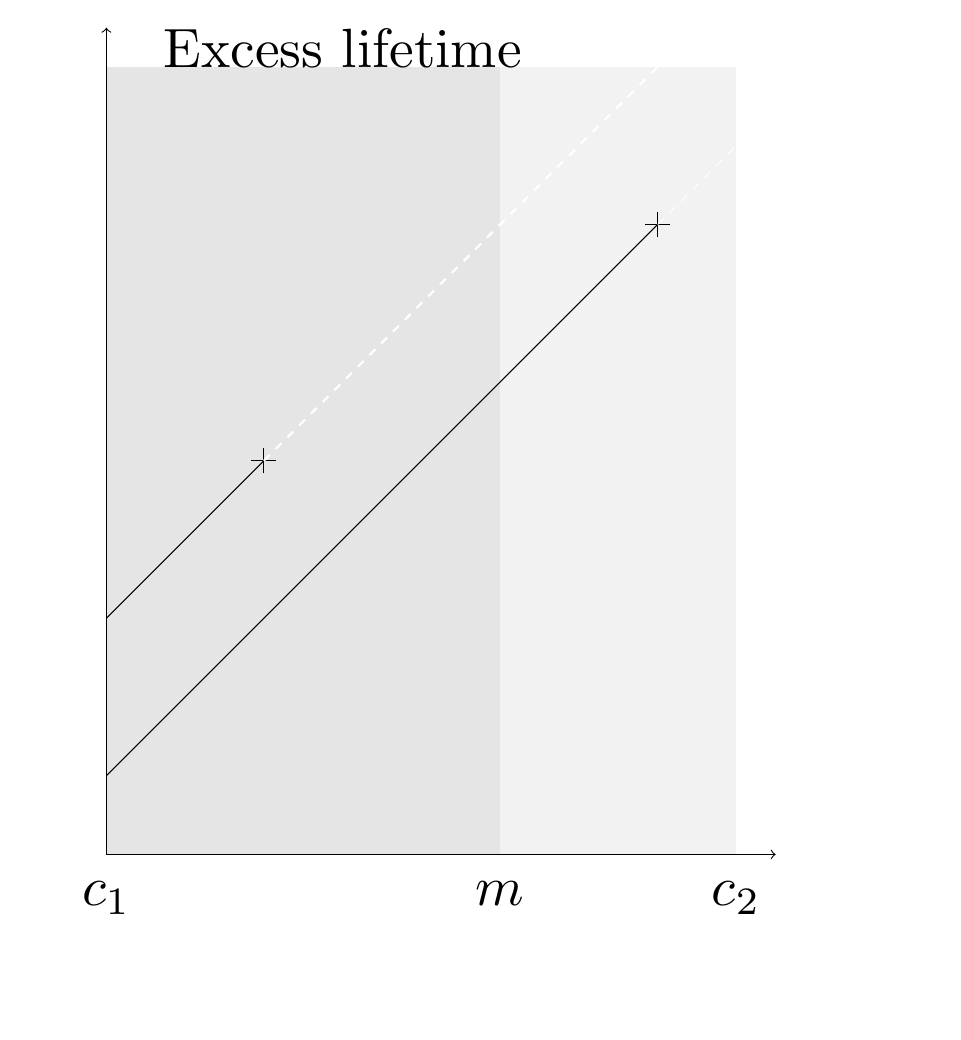
\begin{tikzpicture}[ every node/.style={scale=2}]
\path[clip] (-6,-2) rectangle (5.5,10.5);
\fill [gray!20] (-5,0) rectangle (0,10);
\fill [gray!10] (0,0) rectangle (3,10);
\draw[->](-5,0) -- (3.5,0);
\draw[->](-5,-0) -- (-5, 10.5);
\draw(-5,1) -- (2,8)  node[cross,rotate=45] {};;
\draw[dashed, color = white](2,8)--(4,10);
\draw(-5,3) -- (-3,5)  node[cross,rotate=45] {};;
\node[left] at(-5,0){\footnotesize };
\draw[dashed, color = white, thick](-3,5)--(2,10);
\node[below] at(-5,-0.1) {$c_1$};
\node[below] at(3,-0.1) {$c_2$};
\node[below] at(0,-0.1) {$m$};
\node[anchor=base,inner sep=0pt, outer sep=0pt] at (-2,10) {Excess lifetime};
\end{tikzpicture}
}}
